\section{Coarse preconditioner : the multigrid solver}

Let us first present the coarse part of the preconditioner. It consists of solving the problem on the mesh using an interpolation of degree $p=1$ with a geometric multigrid method. 

Since in general we use an interpolation degree $p$, the first thing to do is to restrict this residual on the same mesh but for a degree $p=1$. The first part of this section presents the restriction used. Similarly, once we have computed the solution for $p=1$, we have to prolong it to a higher degree. To preserve the symmetry of the problem, we will define the prolongation operator to be the transpose of the restriction operator. The procedure explained here is an application with hanging nodes of the one described in \cite{remacle}. Formally, if we denote by $S$ the restriction operator and by $G$ the geometric multigrid solver, we have : 

$$P^cr = S^TGSr$$

The second part explains in more details what are the key components of the geometric multigrid solver. The practical implementation and the way it works with p4est is however described in the next chapter. 

We have to note that the coarse preconditioner cannot be use as the only preconditioner for the CG. Indeed, because of the restriction, it has a kernel, i.e. it is possible to have a high degree residual $r\neq 0$ such that : 

$$Sr = 0$$

As a result, the PCG will stop even tough we have not reached the solution. That is why, in the results chapter, we never test the multigrid alone with a degree superior to $p=1$. 

\subsection{Restriction of $r$ from a high degree to $p=1$}

Let us now define the operator $S$ that will restrict the high degree residual $r$ to a low degree $p=1$. Authors of \cite{l2proj} have shown that a good choice for the restriction is the $L^2$ projection. 

Let us call $V^h_p \subset H^1(\Omega)$ the space whose basis consists of the high degree global basis functions (later denoted $\phi_i$ for $i=1,...,N$) and $V^h_1 \subset H^1(\Omega)$ the one whose basis is constituted by the bilinear global basis function (later denoted $\Phi_i$ for $i=1,...,M$). We want to find $R \in V^h_1(\Omega)$ such that $R$ is the $L^2$ projection of $r \in V^p(\Omega)$ onto $ V^h_1(\Omega)$. As shown in \cite{remacle}, the $L^2$ projection is then given by :

$$ R = Cm^{-1}r$$ 

Where $m$ is the high degree mass matrix and $C$ is called the correlation matrix. The mass matrix $m$ is easy to invert since in the case of spectral elements, it is diagonal, i.e. we have :

\begin{align*}
m_{ij} &= \int_\Omega \phi_i\phi_j \: dxdy \approx 0  &\text{if $i\neq j$}
\end{align*}

%\begin{align*}
%\int_\Omega \phi_i\phi_j \:dxdy &= \sum_{e} \int_{\Omega_e} \phi_i\phi_j \:dxdxy\%\
%&=  \sum_{e} \int_{\Omega_e} \left(\sum_{a=0}^p\sum_{b=0}^p R^e_{ab}(i)l_al_b%\right) \left( \sum_{c=0}^p\sum_{d=0}^p R^e_{cd}(j)l_cl_d\right) \: dxdy\\
%&\approx \sum_e \sum_{m=0}^p\sum_{n=0}^p w_mw_n |J^e_{mn}| %\left(\sum_{a=0}^p\sum_{b=0}^p R^e_{ab}(i)\delta_{am}\delta_{bn}\right) \left( %\sum_{c=0}^p\sum_{d=0}^p R^e_{cd}(j)\delta_{cm}\delta_{dn}\right)\\
%&= \sum_e \sum_{m=0}^p\sum_{n=0}^p w_mw_n |J^e_{mn}|  R_{mn}^e(i)R_{mn}%^e(j)
%\end{align*}

The other term is the correlation matrix. It is defined by : 

$$ C_{I,i} = \int_\Omega \Phi_I\phi_i \: dxdy$$

We can also define its local counterpart using local shape functions. Let us denote $l_i$ the one dimensional shape function of degree $p$ associated with the $i$-th GLL node and $L_i$ the one dimensional linear shape function associated with the $i$-th GLL node. Then we have :

$$ C_{IJ,ij;e} = \int_{\Omega_e} L_IL_J l_il_j \: dxdy$$

If we use the GLL quadrature using the $(p+1)^2$ GLL nodes on quadrant $e$, we get : 

$$C_{IJ,ij;e} \approx w_iw_j|J^e_{ij}| \Phi_I(\xi_i)\Phi_J(\xi_j)$$

For later purposes, let us define : 

\begin{align*}
m_{ij;e} &= w_iw_j|J^e{ij}|\\
B_{IJ,ij} &= \Phi_I(\xi_i)\Phi_J(\xi_j)
\end{align*}

We can then compute the restriction of $r$ as : 

\begin{align*}
y &= m^{-1}r\\
R &= Cy
\end{align*}

Applying $m^{-1}$ to $r$ is rather easy : we only scale the residual by the inverted mass matrix. We now have to transfer $y_i$ for $i=1,...,N$ onto each local quadrant $e$. For this, let us use the operator $R^e_{ij}$ to handle hanging nodes : 

$$ y_{ij;e} = \sum_{K=1}^N R^e_{ij}(K) y_K$$

Let us then compute the local coarse grid residual using the correlation matrix in its local form. This yields :

$$R_{IJ;e} = \sum_{i=0}^p\sum_{j=0}^p B_{IJ,ij}m_{ij;e}y_{ij;e}$$

The last remaining thing to do is to gather the local coarse grid residual to obtain the global coarse grid residual. Let us do not forget to handle the hanging nodes and therefore to use the operator $R^e_{IJ}$ (not to confuse with $R_{IJ;e}$ the local coarse grid residual on quadrant $e$). Let us note that it is not the same as $R^e_{ij}$ since it works on the global nodes for bilinear interpolation where $R^e_{ij}$ is used for the interpolation of degree $p$. 

$$ R_K = \sum_e \sum_{I=0}^1\sum_{J=0}^1 R^e_{IJ}(K) R_{IJ;e}$$

This residual $R$ is then used as a right-hand side for the multigrid solver. 

\subsection{Prolongation of the solution from $p=1$ to a high degree}

Let us assume that the solution given by the multigrid solver with $R$ as right-hand side is given by $Z$, i.e. : 

$$ Z = GR$$

We now need to prolong this coarse scale correction onto the fine grid. Since the prolongation operator is defined as the transpose of the restriction operator, we have : 

$$P^cr = m^{-1}C^TZ$$

The global coarse correction $Z$ is first scattered to each element to have the local coarse scale correction. Let us not forget to handle hanging nodes : 

$$Z_{IJ;e} = \sum_{K=1}^M R_{IJ}^e(K) Z_K$$

Then, let us prolong the correction to obtain :

$$z_{ij;e} = \sum_{I=0}^1\sum_{J=0}^1 B_{IJ,ij}m_{ij;e}Z_{IJ;e}$$

We then have to gather $z_{ij;e}$ to compute its global counterpart. Once again, this is where we handle hanging nodes.

$$z_{K} = \sum_e\sum_{i=0}^p\sum_{j=0}^p R^e_{ij}(K)z_{ij;e}$$

The last thing left to do is to scale $z_K$ by the inverted mass matrix. This yields : 

$$(P^cr)_K = \frac{z_K}{m_K}$$

\subsection{The geometric multigrid solver}

This subsection generally describes how the geometric multigrid method works and why it is so efficient. However, a lot of details have been omitted and more information can be obtained in the relevant literature (for example in \cite{multi_book}). It has to be noted that here the degree of interpolation is always $p=1$.

\subsubsection{Motivation}

The first observation we have to make is that for any known function $v$ such that $v(x,y)=u_0$ if $(x,y) \in \Gamma$, we can rewrite problem \ref{eq:poisson}. Indeed, if we define a function $e = u-v$, then we have

\begin{align}
\nabla ^2 e &= f-\nabla^2v = r &\text{on $\Omega$} \label{eq:poisson_error}\\
e &= u-v = 0 &\text{on $\Gamma$}
\end{align}

Which is qualitatively the same problem. But if we are able to solve it for $e$ more easily than we would have been able to do it for $u$, then we can simply recover $u$ from $e$ : 

$$u = v + e$$

The second observation we have to make is that the discretization of problem \ref{eq:poisson} or equivalently the one above yields a linear system of equations to solve (as the one derived in the first section of this chapter). As already mentioned, the matrix $A$ defining this linear system has very often a very large condition number $\kappa(A)$. As a result, using iterative methods can be very slow. Typically, the condition number of $A$ for $p=1$ is $\mathcal{O}(h^2)$ where $h$ is the size of the smallest quadrant (see \cite{condNumb}). Thus, if we use a coarser grid (where the smallest quadrant has a larger size than before), the problem is easier to solve. 

The idea behind multigrid is therefore a two-level idea. It works as follow : 

\begin{enumerate}
\item Given an approximate solution to the problem, compute the residual $f-\nabla^2v$.
\item Solve problem \ref{eq:poisson_error} to obtain $e$. It should be easier to solve than the initial problem by using a coarser grid.
\item Add $e$ to $v$ to get the solution $u$. 
\end{enumerate}

The next step in the reasoning is to use this idea recursively. Indeed, in step 2, to solve problem \ref{eq:poisson_error}, one can reuse the same process. A more precise definition of the algorithm is given at the end of this section, in algorithms  \ref{mu_cycle} and \ref{multi_algo}.

We still have not explained two things in the procedure above. The first is how to choose an approximate solution to the problem. In theory, it can be any but we have to remember that, in step 2, we will use a coarser grid to solve for $e$. As a result, we want an approximation such that $e = u-v$ is a smooth function that a coarse grid can capture well. One way to obtain this approximation is by using an iterative method. Indeed, it has been shown (for example, in \cite{smoothing}) that even tough iterative methods like Jacobi or Gauss-Seidel have a tendency to stall, just a few iterations allows them to capture the high-frequency modes in the solution. That means that if we compute $v$ by doing some iterations of the Jacobi method, then $e = u-v$ will contain only low frequency modes. And a solution containing low frequencies can be computed on a coarser grid. This property that the high frequency errors converge a lot quicker than the low frequency error is called the smoothing property and is hold by a lot of different smoother (for example, the Jacobi method).

The second thing we have to consider is how to transfer one function onto another grid. Indeed, in step 1, we compute the residual $f-\nabla^2 v$ but then we have to solve problem \ref{eq:poisson_error} on a different, coarser grid. We therefore need an operator to compute the right-hand side of the linear system on the coarser grid from the right-hand side of the one on the initial grid. This is called the restriction operator. Similarly, when we have computed the solution on the coarser grid in step 2, we need to update our approximation $v$ with $e$ on the initial grid. This operator is called the prolongation operator. We will see that there exists a link between those two operators.

\subsubsection{The smoother : damped Jacobi method}

Let us now present the smoother used : the damped Jacobi method. Let us assume that we want to solve :

$$Av=b$$

Let us then split the matrix $A$ in the form : 

$$(D-L-U)v = b$$

Where $D$ is a diagonal matrix containing the diagonal of $A$, $-L$ is the strictly lower triangular part and $-U$ is the strictly upper triangular part. Let us also denote as $v^i$ the approximation of the solution of $Av=b$ after the $i$-th iteration. Then, the damped Jacobi method with damping factor $\omega$ is given by : 

$$ v^{i+1} = \omega\left(D^{-1}(L+U)v^i + D^{-1}b\right) + (1-\omega)v^i$$

It is to be noted that since $D$ is diagonal, it is very cheap to compute $D^{-1}$. It can be shown (see \cite{multi_book}) that if $0<\omega\leq 1$ then the damped Jacobi method is stable. The parameter $\omega$ can then be tuned to obtain different properties in the convergence of high frequency errors. In \cite{multi_book}, it is shown that a good choice for $\omega$ is : 

$$\omega = \frac{2}{3}$$

We now have to explain how to compute $A$ for the different grids. Since it results from the discretization of problem \ref{eq:poisson_error}, we can use the same method as the one explained in the section concerning the spectral element method. It is here even easier since we have piece-wise bilinear global basis function. We however still have to be careful of hanging nodes. The next chapter explains in more details the implementation. 

\subsubsection{Prolongation operator}

Let us now define the prolongation operator, i.e. the operator that takes the solution to problem \ref{eq:poisson_error} on the coarse grid and prolong it on the fine grid. 

\begin{figure}
\centering
\begin{subfigure}{.5\textwidth}
  \centering
  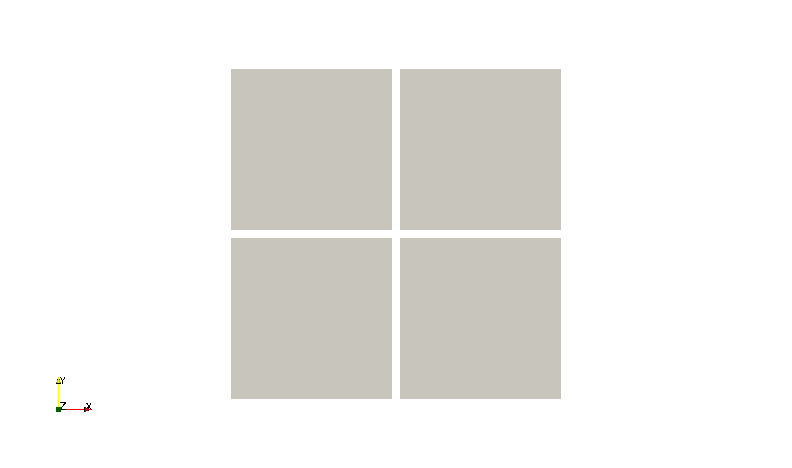
\includegraphics[width=1.2\linewidth]{Theory/hang_lev_1.png}
  \caption{Mesh at level 1}
  \label{hang_lev_1}
\end{subfigure}%
\begin{subfigure}{.5\textwidth}
  \centering
  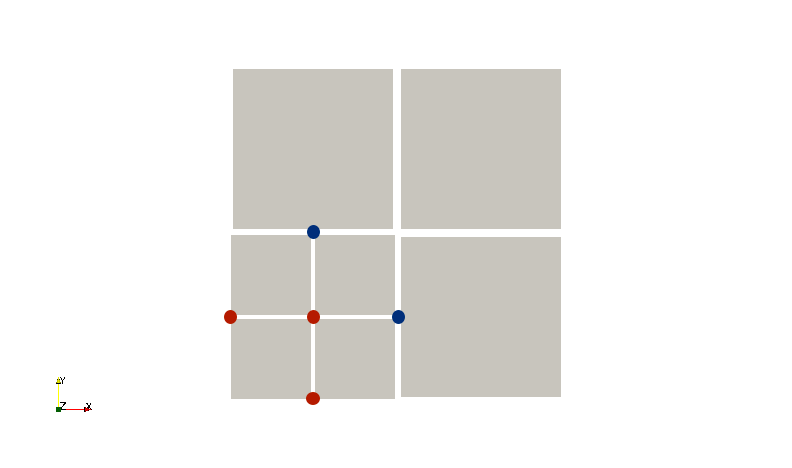
\includegraphics[width=1.2\linewidth]{Theory/hang_lev_2.png}
  \caption{Mesh at level 2}
  \label{hang_lev_2}
\end{subfigure}
\caption{Example of two meshes used in the geometric multigrid method. The one on the left is the coarser mesh, where all quadrants have a refinement level of 1. The one on the right has some quadrants that have a level of refinement of 2 and is therefore the level 2 mesh. We can also see the influence of increasing by one level. We have the apparition of three new global nodes (in red) and two new hanging nodes (in blue).}
\label{hang_lev}
\end{figure}

In order to do this, we have to precise the nature of the different meshes that will be used. As explained earlier, we will solve the problem on different meshes. Let us organize those meshes on different levels, where the lowest level has the coarsest mesh and the highest level has the finest mesh.  The AMR provides us with a natural choice for the definition of those meshes. Indeed, since each quadrant is dynamically refined, we will consider the mesh at level $lev$ to be the original mesh where the maximum level of refinement is $lev$ (see for example \cite{levelMulti}). An example is given on figure \ref{hang_lev}. We can see that the mesh on the left has all its quadrants with a refinement level of 1, it is thus the mesh at level 1. On the right, the mesh has some (but not all) quadrants that have a refinement level of 2. It is therefore the mesh at level 2. 

Now that we have some sense of how the meshes are constructed, it is possible to define the prolongation operator. We can see on figure \ref{hang_lev_2} the influence of increasing by one level. There is the apparition of three new global nodes (in red) and two new hanging nodes (in blue).

Since we use a bilinear interpolation (thus linear along each edge), the prolongation operator is quite natural : the new node created in the middle of a refined quadrant (and that can never be hanging) is equal to a fourth of the sum of the values at the corners of the larger quadrant. Concerning the nodes added on the edges, if they are not hanging, they are equal to half of the sum of the values at the ends of the edge. Of course, we do not need to compute the prolongation for the hanging edges since they are not global. 

\subsubsection{Restriction operator}

As before, to conserve the symmetry of the problem, the restriction operator is defined as the transpose of the prolongation operator. 

It means that if a group of four quadrants has to be coarsened to move to the mesh a level below, the value of the residual at the middle node (once again, it can never be hanging) contributes a fourth of its value to the residual at the four corners of the larger quadrant. Similarly, the residual at a node on an edge that is not hanging contributes half of its value to both nodes at the ends of the edge. 

\subsubsection{Formalization of the algorithm}

In this last part, we will give the pseudo-code for the geometric multigrid solver. Let us denote $A^{lev}$ the matrix arising form the discretization on the mesh at level $lev$, $I_{lev}^{lev+1}$ the prolongation operator, $I_{lev+1}^{lev}$ the restriction operator, $v^{lev}$ the value of the solution at level $lev$ and $r^{lev}$ the value of the right-hand side at level $lev$.

\begin{algorithm}
\begin{algorithmic}
\Function{M$\mu$}{$v^{lev}$,$r^{lev}$}
\If{$lev=0$}
	\State Solve $A^0v^0 = r^0$ using a direct method
\Else
	\State Do $\nu_1$ iterations of the damped Jacobi method on $A^{lev}u = r^{lev}$
	\State $r^{lev-1} = I_{lev}^{lev-1}r^{lev}$
	\State $v^{lev-1} = 0$
	\State $v^{lev-1} = M\mu(v^{lev-1},r^{lev-1})$ \text{ $\mu$ times}
	\State $v^{lev} = v^{lev} + I_{lev-1}^{lev}v^{lev-1}$
	\State Do $\nu_2$ iterations of the damped Jacobi method on $A^{lev}u = r^{lev}$
\EndIf	
\Return $v^{lev}$
\EndFunction
\end{algorithmic}
\caption{$\mu$-cycle scheme}
\label{mu_cycle}
\end{algorithm}


Algorithm \ref{mu_cycle} describes what is called a $\mu$-cycle scheme. We can see several parameters in this algorithm. First, the number of times we recursively use the function, $\mu$. In practice, only $\mu=1$ (called a V-cycle) and $\mu=2$ (called a W-cycle) are used. We also have the number of smoothing iterations we do before restricting the residual, $\nu_1$, called the pre-smoothing parameter and the number of smoothing iterations we do after the correction, $\nu_2$, called the post-smoothing parameter. 

The last thing to say is that we can use the $\mu$-cycle scheme as an iterative process, each iteration being one $\mu$-cycle. Algorithm \ref{multi_algo} describe how the procedure works to solve the problem defined by $Au=b$.

\begin{algorithm}
\begin{algorithmic}
\State $v = 0$
\State $r = b-Av$
\For{$i=0,1,...$}
\State $e = 0$
\State $e = M\mu(e,r)$
\State $v = v + e$
\State $r = b-Av$
\EndFor
\end{algorithmic}
\caption{Geometric multigrid solver}
\label{multi_algo}
\end{algorithm}

An important characteristic of geometric multigrid methods is the h-independent convergence. To obtain a given tolerance of the norm of the residual $r$, the number of iterations needed in algorithm \ref{multi_algo} remains constant for any number of levels. Of course, the time needed to perform an iteration increases if we have more levels but the number of iterations remains identical. 














